\scanpage{27}
% archive sheet number: 26

cette dernière relation $\Sigma_1^-\cap\Sigma_2^-\ne\varnothing$ est vraie
$=$ si $E_1=E_2=\varnothing$, car
\deleted{\unsure{donc|alors} par hyp.} si on avait de plus
$\Sigma_1^-\cap\Sigma_2^-=\varnothing$, on en conclurait que les deux
\deleted{part.} décompositions binaires \deleted{\unsure{son|sont}}
(qui sont alors des partitions binaires) sont \uline{identiques},
ce que l'on \inserted{a} exclu. Cela montre que les
$\Sigma_1^+,\Sigma_2^+$ sont uniquement déterminés.

On a donc le diagramme d'inclusions
\diagram{\begin{tikzcd}[ampersand replacement=\&,column sep=small]
\Sigma_1^+ \& E_1 \arrow[l,hook] \arrow[r,hook] \& \Sigma_{12}
\& E_2 \arrow[l,hook] \arrow[r,hook] \& \Sigma_2^+
\end{tikzcd}}
qu'on, exprime par un diagramme
\figure{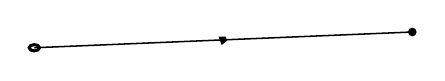
\begin{tikzpicture}[x=1cm,y=1cm]
\draw[line width=.55pt] (0,0) -- (2.4,.10) -- (4.8,.20);
\draw[line width=1.1pt] (0,0) ellipse [x radius=.065,y radius=.040];
\fill (2.34,.14) -- (2.43,.14) -- (2.45,.09) -- (2.38,.035) -- cycle;
\fill (4.8,.20) circle [radius=.055];
\end{tikzpicture}}
\diagram{\begin{tikzcd}[ampersand replacement=\&,column sep=small]
\Sigma_1^+ \& E_1 \arrow[l,hook] \arrow[r,hook] \& \Sigma_{12}
\& E_2 \arrow[l,hook] \arrow[r,hook] \& \Sigma_2^+
\end{tikzcd}}

\margin{\[
\text{NB}\left\{\begin{aligned}
\Sigma_1^-&=\Sigma_{12}\amalg_{E_2}\Sigma_2^+\\
\Sigma_{\deleted{\unsure{1}}2}^-&=\deleted{\unsure{E}}\Sigma_{12}\amalg_{E_1}\Sigma_1^+
\end{aligned}\right.
\]}

\margin{Ceci n'implique pas que les quatre ensembles
$\Sigma_1^+,\Sigma_1^-,\Sigma_2^+,\Sigma_2^-$ soient distincts,
car on peut avoir (non pas $\Sigma_1^+=\Sigma_2^+$,
ni $\Sigma_1^-=\Sigma_2^-$, mais) $\Sigma_1^+=\Sigma_2^-$,
qui équivaut à $E_1=\Sigma_{12}$ et entraîne $E_2=\varnothing$
(cela signifie, en termes des $(\Sigma_1^+,\Sigma_1^-)$ que
$\Sigma_2^{\unsure{\dot{-}|-}}=\Sigma_1^+$,
$\Sigma_2^+=X\setminus\Sigma_1^+=\overset{\unsure{\circ|\leftarrow}}{\Sigma}{}_1^{-,\unsure{\circ|0}}$)
\deleted{\unsure{ou}} et la relation \unsure{symetrique|symétrique}.
On ne veut pas exclure ce cas, i.e.\ \deleted{\unsure{nous|mais}}
n'exigeons pas que les quatre ensembles
$\Sigma_1^+,\Sigma_1^-,\Sigma_2^+,\Sigma_2^-$ soient distincts
s'ils le \unsure{\deleted{sont}|sont}, on dit que les
\deleted{\unsure{ens.}} \inserted{deux décomp. bin.}
\deleted{\unsure{sont strictmt|sont strict.}} non parallèles.}

Je me propose d'étudier les ensembles finis
\unsure{indicellés|indiciellés}
$\deleted{\unsure{\Sigma|\Pi}}(\unsure{\Pi|\pi}_\alpha)_{\alpha\in A}
\deleted{=(\unsure{\Sigma_\alpha^i}),\unsure{\alpha\in A}}$
$\deleted{\Pi_\alpha=\{\Sigma_\alpha^\varepsilon}$
de décompositions binaires de $\unsure{X}$ deux à deux non parallèles.

Voici une façon très \unsure{générale|génerale}
d'\deleted{en}obtenir des floppées.
